\documentclass[12pt, letterpaper]{article}
\usepackage{graphicx} % Required for inserting images
\usepackage{hyperref}
\usepackage{listings}
\usepackage{amssymb}
\usepackage{amsmath}
\usepackage[english]{babel}
\usepackage{nicefrac, xfrac}
\usepackage{mathtools}
\newcommand{\acc}{\\\hphantom{}\\}
\usepackage[table,xcdraw]{xcolor}
\usepackage[paper=a4paper,left=20mm,right=20mm,bottom=25mm,top=25mm]{geometry}
\renewcommand{\labelenumii}{\arabic{enumi}.\arabic{enumii}}
    \renewcommand{\labelenumiii}{\arabic{enumi}.\arabic{enumii}.\arabic{enumiii}}
    \renewcommand{\labelenumiv}{\arabic{enumi}.\arabic{enumii}.\arabic{enumiii}.\arabic{enumiv}}
\title{Ristrutturazione Università 2}
% \author{ Giacomo Biribicchi \and Marco Casu \and Christian Di Manno \and Alessandro Gautieri }
\date{}


\begin{document}

\maketitle




\section{Tipi di Dato e Domini}
\subsection{Domini}
\begin{itemize}
    \item create domain $Intger>0$ as integer
    default 0
    check $(value>=0);$
\end{itemize}
\subsection{Tipi}
\begin{itemize}
    \item 
\end{itemize}


CF = [A-Z]\{6\} [0-9]\{2\} [A-Z]\{1\} [0-9]\{2\} [A-Z]\{1\} [0-9]\{3\} [A-Z]\{1\}\acc 

\section{Vincoli Esterni}
\begin{itemize}
    \item $\lnot \exists s,p,v Studente(s) \and Professore(p) \land cf(s,v) \and cf(p,v)$
\end{itemize}
\section{UML}
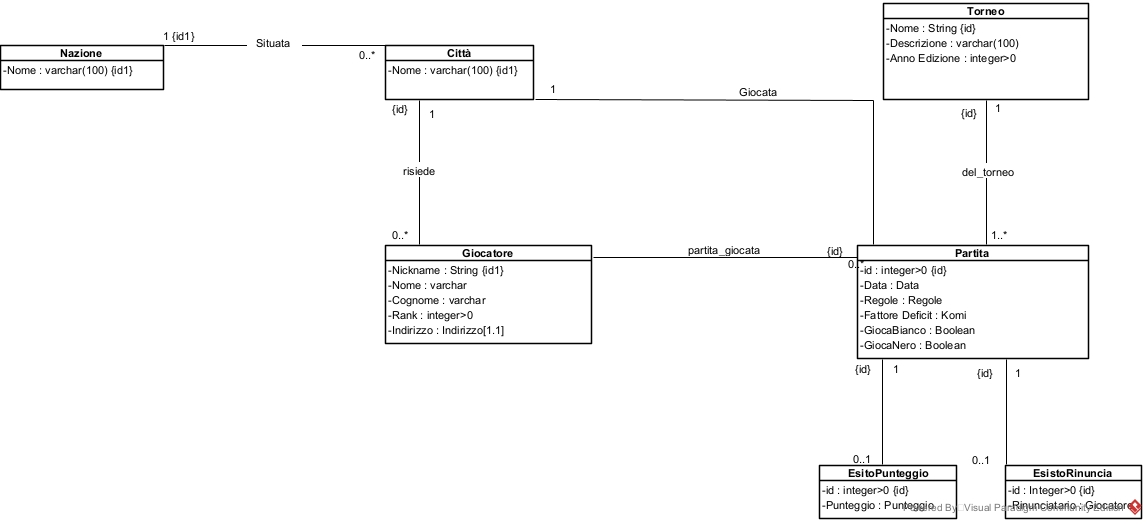
\includegraphics[width=\textwidth]{UML.jpg}


\end{document}